\documentclass[11pt]{article}

\usepackage[letterpaper,margin=1.15in,top=1in,bottom=1.1in]{geometry}
\usepackage[T1]{fontenc}
\usepackage{lmodern}
\usepackage{microtype}
\usepackage{amsmath,amssymb}
\usepackage{booktabs}
\usepackage{tabularx}
\usepackage{enumitem}
\usepackage{xcolor}
\usepackage{titlesec}
\usepackage{fancyhdr}
\usepackage{tcolorbox}
\usepackage{graphicx}
\usepackage{listings}
\usepackage{tikz}
\usetikzlibrary{arrows.meta,positioning}
\usepackage[hidelinks]{hyperref}

\definecolor{mitred}{HTML}{8C1D1D}
\definecolor{soft}{HTML}{F6F2F2}
\definecolor{ink}{HTML}{222222}
\definecolor{midgrey}{HTML}{555555}
\definecolor{codebg}{HTML}{F7F7F5}
\definecolor{comment}{HTML}{6E7781}

\titleformat{\section}{\large\bfseries\color{mitred}}{\thesection.}{0.55em}{}
\titleformat{\subsection}{\normalsize\bfseries\color{ink}}{\thesubsection}{0.55em}{}
\titlespacing*{\section}{0pt}{1.6em}{0.6em}
\titlespacing*{\subsection}{0pt}{1.1em}{0.4em}

\pagestyle{fancy}\fancyhf{}
\lhead{\small\color{mitred}Autoresearch \textbullet{} An Agent That Improves a Number}
\rhead{\small\thepage}
\renewcommand{\headrulewidth}{0.4pt}

\setlist[itemize]{leftmargin=1.2em,itemsep=3pt,topsep=4pt}
\setlist[enumerate]{leftmargin=1.5em,itemsep=3pt,topsep=4pt}

\newtcolorbox{idea}[1][]{colback=soft,colframe=mitred,boxrule=0.9pt,
  left=8pt,right=8pt,top=6pt,bottom=6pt,arc=2pt,#1}
\newtcolorbox{aside}[1][]{colback=white,colframe=midgrey,boxrule=0.5pt,
  left=8pt,right=8pt,top=6pt,bottom=6pt,arc=2pt,#1}

\newcommand{\keyidea}[1]{\begin{idea}#1\end{idea}}
\linespread{1.07}

\lstdefinestyle{code}{
  basicstyle=\ttfamily\small,
  backgroundcolor=\color{codebg},
  commentstyle=\color{comment}\itshape,
  keywordstyle=\color{mitred},
  showstringspaces=false,
  breaklines=true,
  frame=none,
  xleftmargin=10pt,
  framexleftmargin=10pt,
  aboveskip=10pt, belowskip=6pt,
}
\lstset{style=code}
\lstdefinelanguage{pseudo}{morekeywords={repeat,if,stop,return},morecomment=[l]{\#}}
\definecolor{taskbg}{HTML}{E7EEF7}
\definecolor{sandbg}{HTML}{E6F1EA}
\definecolor{handbg}{HTML}{F2F2F0}
\definecolor{taskink}{HTML}{1F4E79}
\definecolor{sandink}{HTML}{1D6B52}

\lstdefinestyle{pbase}{basicstyle=\ttfamily\footnotesize, breaklines=true,
  xleftmargin=10pt, framexleftmargin=10pt, aboveskip=0pt, belowskip=0pt,
  escapeinside={(*@}{@*)}}
\lstdefinestyle{prompt}{style=pbase, backgroundcolor=\color{handbg}}
\lstdefinestyle{ptask}{style=pbase, backgroundcolor=\color{taskbg}}
\lstdefinestyle{psand}{style=pbase, backgroundcolor=\color{sandbg}}
\lstdefinestyle{promptwide}{style=ptask, basicstyle=\ttfamily\scriptsize,
  escapeinside={(*@}{@*)}}

% derived values appearing inside an otherwise hand-written sentence
\newcommand{\dt}[1]{\textcolor{taskink}{\bfseries #1}}
\newcommand{\ds}[1]{\textcolor{sandink}{\bfseries #1}}
\newcommand{\swatch}[1]{\raisebox{-0.5pt}{\fcolorbox{midgrey!50}{#1}{\rule{0pt}{5.5pt}\rule{7pt}{0pt}}}}

\newcommand{\runin}[1]{\smallskip\noindent\textbf{#1}\quad}
\newcommand{\from}[1]{\vspace{-2pt}\par\noindent\hspace*{12pt}%
  \begin{minipage}{\dimexpr\linewidth-14pt\relax}
  {\small\color{midgrey}$\hookleftarrow$~\itshape #1}
  \end{minipage}\par\smallskip}

\begin{document}

\begin{center}
{\LARGE\bfseries\color{mitred} An Agent That Improves a Number}\\[0.4em]
{\large\color{mitred} Design note}\\[0.6em]
{\small\color{midgrey} github.com/Vivekf/autoresearch}
\end{center}

\vspace{0.5em}\hrule height 0.9pt\vspace{1.2em}

\noindent
We start with the shape of research itself, then build the four things a machine needs in order
to do it, and finish by assembling them into the only artifact the agent ever actually reads:
about thirty lines of text.

\keyidea{\textbf{The whole lecture in one line.} Give an agent a number and tell it to make the
number better. What it does next is the subject.}

% =====================================================================
\section{How research gets done}

\subsection{The cycle}

Strip research of its trappings and a loop is left. You have a question. You form a guess about
what might improve the answer. You build something concrete enough to try. You measure it. And
the measurement changes your next guess.

\begin{lstlisting}[language=pseudo]
state <- what I know so far

repeat:
    hypothesis <- propose(state)       # what might make it better?
    experiment <- build(hypothesis)    # make it concrete enough to run
    result     <- measure(experiment)  # a number I did not get to choose
    state      <- state + (hypothesis, result)
\end{lstlisting}

The third line is what separates research from guessing. A result you chose is a decoration; a
result you did not choose can contradict you. Much of this lecture is in service of making that
line real --- of building a measurement the agent genuinely cannot influence.

\subsection{The same cycle, mechanised}

An agent is a prompt in a loop. What changes between one agent and another is what is in its
hands --- and with the right two tools, the cycle above \emph{is} the agent loop.

\begin{lstlisting}[language=pseudo]
repeat:
    code    <- model(context)       # propose and build, in one step
    output  <- sandbox.run(code)    # stdout, or a traceback
    score   <- scorer.score()       # the measurement it does not control
    context <- context + [code, output, score]
\end{lstlisting}

\noindent Notice that \emph{propose} and \emph{build} have collapsed into a single step. For a
model that writes programs, having the idea and expressing it are the same act --- which is a
large part of why any of this works.

\subsection{The same cycle, as code}

Close to what actually runs, with the bookkeeping stripped out.

\begin{lstlisting}[language=Python]
def run_agent(goal, max_turns=60):
    messages = [{"role": "system", "content": PROMPT},
                {"role": "user",   "content": goal}]

    for turn in range(max_turns):
        reply = client.chat.completions.create(
            model=MODEL, messages=messages, tools=TOOLS
        ).choices[0].message

        if not reply.tool_calls:           # asked for nothing -> it is done
            return reply.content

        messages.append(reply)             # what it decided to do

        for call in reply.tool_calls:
            args   = json.loads(call.function.arguments)
            result = TOOL_FUNCTIONS[call.function.name](**args)
            messages.append({"role": "tool",
                             "tool_call_id": call.id,
                             "content": str(result)})
\end{lstlisting}

\runin{There is no research in it.}
No planning, no hypothesis, no decision about what to try next. Every one of those happens
inside \texttt{client.chat.completions.create}. The function around it is a courier.

\runin{The two \texttt{append} lines are the whole mechanism.}
Strip them out and the model begins again from nothing every turn, with no memory of what it
tried or what happened. Put them back and you have an agent.

\keyidea{The loop is a \textbf{context-accumulation machine}, and the accumulation is the
intelligence.}

\subsection{What is ours to design}

Three things, and only three: \textbf{what tools exist}, \textbf{what goes into the context},
and \textbf{what ends the loop}. Everything else is downstream of those.

The third is worth sitting with. The loop exits when the model stops asking for tools --- nobody
wrote a rule about when a research project is finished. \texttt{max\_turns} is a safety belt, not
a design parameter. Whether that is a sensible way to end a piece of research is one of the
questions this lecture exists to ask.

% =====================================================================
\section{What the loop needs}

Four things, in the order the loop needs them: a \textbf{problem}, a definition of
\textbf{better}, a \textbf{measurement}, and somewhere to \textbf{run experiments}.

\begin{center}
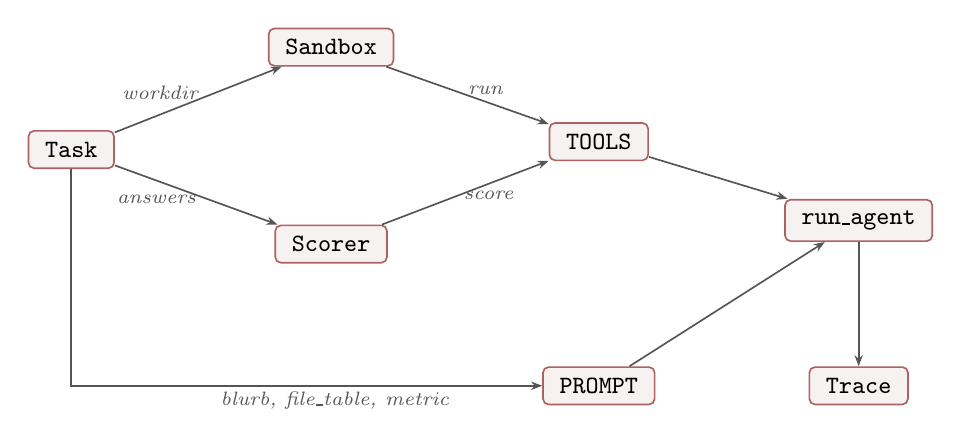
\begin{tikzpicture}[
  box/.style={draw=mitred!70, rounded corners=2pt, fill=soft, inner xsep=6pt, inner ysep=4pt,
              font=\ttfamily\small},
  lab/.style={font=\scriptsize\itshape, color=midgrey, inner sep=2pt},
  every path/.style={->, >={Stealth[length=4pt,width=3pt]}, draw=midgrey, semithick}
]
  \node[box] (task) at (0,0.6)      {Task};
  \node[box] (sand) at (3.3,1.9)    {Sandbox};
  \node[box] (scor) at (3.3,-0.6)   {Scorer};
  \node[box] (tool) at (6.7,0.7)    {TOOLS};
  \node[box] (prom) at (6.7,-2.4)   {PROMPT};
  \node[box] (loop) at (10.0,-0.3)  {run\_agent};
  \node[box] (trac) at (10.0,-2.4)  {Trace};

  \draw (task) -- node[lab, above left=-3pt] {workdir} (sand);
  \draw (task) -- node[lab, below left=-3pt] {answers} (scor);
  \draw (task.south) |- node[lab, below, pos=0.78] {blurb, file\_table, metric} (prom.west);
  \draw (sand) -- node[lab, above right=-3pt] {run}   (tool);
  \draw (scor) -- node[lab, below right=-4pt] {score} (tool);
  \draw (tool) -- (loop);
  \draw (prom) -- (loop);
  \draw (loop) -- (trac);
\end{tikzpicture}
\end{center}

\noindent{\small\itshape The one edge not drawn: \texttt{Sandbox} also contributes its execution
model and package list to \texttt{PROMPT}, so the instructions always describe the environment
the agent is really in.}

% ---------------------------------------------------------------------
\subsection{\texttt{Task} --- what is being asked}

\runin{Abstractly.}
A held-out prediction problem. One table of observations, split three ways, with some columns
visible at prediction time and some not. You declare five things:

\begin{center}
\begin{tabularx}{\textwidth}{@{}l X@{}}
\toprule
\texttt{keys} & columns that identify a row --- present in training data \emph{and} at
  prediction time \\
\texttt{features} & columns usable at prediction time \\
\texttt{train\_only} & columns observed historically but unavailable when predicting \\
\texttt{target} & the column to predict \\
\texttt{metric} & how a prediction is judged \\
\bottomrule
\end{tabularx}
\end{center}

\noindent Everything else follows mechanically. The files are \emph{derived} from those roles:

\begin{lstlisting}
train.csv        =  keys + features + train_only + [target]
dev_pairs.csv    =  keys + features
test_pairs.csv   =  keys + features
predictions.csv  =  keys + [prediction]
\end{lstlisting}

\keyidea{The gap between the first line and the second \textbf{is} the task. It is not written
anywhere; it is the arithmetic difference between two column lists. Move a column from
\texttt{train\_only} to \texttt{features} and the problem changes, the files change, and the
prompt changes --- without touching any prose.}

\noindent Then the split: one frame, a seeded permutation, 80/10/10. The training answers go into
the file. The dev and test answers stay in memory and are never written anywhere at all.

The \textbf{seed is the secret}. Not the data --- the data is public. What the agent cannot
reconstruct is \emph{which rows landed in dev}, and that alone is enough to make the held-out set
genuinely held out.

\runin{Concretely.}

\begin{lstlisting}[language=Python]
keys       = ["row_id", "col_id"]   # a user and a movie
features   = []                     # none at prediction time
train_only = ["t"]                  # timestamps, train only
target     = "value"                # the rating, 1-5
metric     = rmse(clip=(1, 5))
\end{lstlisting}

\noindent Three rows of each file, side by side:

\begin{lstlisting}
what the agent is asked:        what we are holding back:
 row_id  col_id                  row_id  col_id  value
   3153    3599                    3153    3599      4
   2690    3167                    2690    3167      3
   3412    3095                    3412    3095      4
\end{lstlisting}

\noindent Two bare integers in, a rating out. There is nothing else in the input, which is
exactly why the task pushes the agent toward matrix completion: the only signal available is the
pattern of \emph{other} ratings by the same row and of the same column.

\begin{aside}
\textbf{Why \texttt{row\_id} and not \texttt{user}.} Underneath this is MovieLens 1M ---
\emph{the} standard benchmark for rating prediction --- so any competent model has read papers
about it and can recall that matrix factorization works well without discovering anything. The
task is therefore \textbf{anonymised}: neutral column names, reshuffled identifiers, no titles or
genres, and a row count that is not the recognisable 1{,}000{,}209. The \emph{structure} survives
on purpose. Reasoning from a sparse table of integers to matrix completion is generalisation;
reciting a leaderboard is not. The switch is what separates them.
\end{aside}

% ---------------------------------------------------------------------
\subsection{\texttt{Metric} --- what ``better'' means}

\runin{Abstractly.}
A name, a function, a direction, and optionally a clamp. The function is the obvious part. The
\emph{direction} is the one that is easy to underrate: \texttt{lower\_is\_better} silently
controls which attempt counts as an improvement worth keeping, whether the leaderboard runs a
running minimum or a maximum, what ``best so far'' means, and which way the gap between dev and
test points.

Get it wrong and the closing number prints backwards. It did, until the harness was pointed at
an accuracy task and reported a \emph{better} test score as evidence of optimism.

The clamp belongs to the task rather than to the metric family --- RMSE does not know that
ratings stop at 5 --- so it is a parameter, not a property.

\runin{Concretely.}
\texttt{rmse(clip=(1,\,5))}. Root mean squared error, lower is better, predictions clamped to the
legal rating range before scoring. The clamp is a small kindness: a model that predicts 5.4 for
an enthusiast is not wrong in a way worth punishing.

% ---------------------------------------------------------------------
\subsection{\texttt{Scorer} --- the measurement, and the deliverable}

\runin{Abstractly.}
Two jobs. The second one is a repair.

\medskip\noindent\textbf{The number.} Read the agent's predictions, line them up against the
held-out answers by \texttt{keys}, refuse if any row is unpredicted, apply the metric. One float.
This is the agent's only sense organ; it has no other way to learn whether an idea was any good.

This object is also the \textbf{trust boundary}. It is the only thing holding both the answers
and the ability to read the agent's output, so the asymmetry is enforced by what each object
\emph{has} rather than by rules anyone has to remember.

\begin{aside}
\texttt{score} is a \emph{tool call}, so the agent cannot invoke it from inside its own Python.
One configuration per turn. That rules out hyperparameter sweeps --- and enforces, by accident,
the discipline of changing one thing at a time and measuring it. One run, denied sweeps, built
itself an internal validation split so it could tune offline and spend its single scoring call on
the winner. That was the best thing any run did, and nobody told it to.
\end{aside}

\medskip\noindent\textbf{The deliverable.} Every attempt writes predictions for the dev pairs
\emph{and} the test pairs. Whenever an attempt turns out to be the best so far, its test
predictions are copied somewhere the agent cannot reach. The agent never decides when to submit.

That job exists because the obvious alternative failed twice. Asking the agent to write its final
answer \emph{``when you are done''} meant one run never judged itself done, ran out of turns and
produced nothing at all --- and another lost track of which model had been its best and shipped a
worse one, reporting 0.8579 while submitting a 0.8616 model.

\keyidea{Coupling the deliverable to the stopping decision was the mistake. Uncoupling them makes
both failures impossible to express.}

\runin{Why there is a dev set \emph{and} a test set.}
This is the idea everything else serves. Every time the agent reads a dev score and chooses what
to try next, it spends a little information about dev. Do that twenty-eight times and dev has
been \emph{fit} --- not by gradient descent, but through a sequence of keep-this, discard-that
decisions. Each one is a parameter update made of judgement instead of derivatives.

\keyidea{The agent is playing the role the optimiser usually plays, and it overfits the
validation set exactly the way an unconstrained hyperparameter search does. Test informed no
decision, so test is the honest number.}

\noindent What the last cell prints:

\begin{lstlisting}
best dev RMSE         0.9815   (over 1 attempts)
submitted from      attempt 1, which scored 0.9815 on dev
test RMSE             0.9843
optimism             +0.0028  (test is worse than dev)
\end{lstlisting}

% ---------------------------------------------------------------------
\subsection{\texttt{Sandbox} --- where experiments happen}

\runin{Abstractly.}
A Python process the agent can send code to, with the task's files as its working directory. Most
of it is plumbing. One decision in it is not.

\keyidea{Whether the process \textbf{persists between calls} sets the price of a marginal
experiment --- and therefore how much research gets done.}

\noindent With a fresh process each time, every attempt pays full freight: reload the data,
rebuild the model, retrain from zero. With a session that stays alive, \emph{``train five more
epochs on the model I already have''} costs three lines and a couple of seconds. The same agent
will do different research depending on which one it has.

Timeouts follow from the same reasoning. The obvious implementation --- kill the process when a
step runs long --- destroys every variable, which punishes precisely the long training runs the
task is supposed to reward. So the interrupt happens \emph{inside} the session: a timer fires,
the step stops, the agent is told, and its variables survive.

The package list is \textbf{probed, not declared}. Colab and a laptop differ, and a prompt that
lies about the environment wastes turns.

\runin{Concretely.}
\texttt{Sandbox(task.workdir, persistent=True, timeout=180)} --- three minutes per step, enough
to fit a factorization on 800k ratings and not enough to sit through a bad idea. It reports
\texttt{numpy, pandas, scipy, scikit-learn}, because that is what it found.

% =====================================================================
\section{The prompt, assembled}

Everything above exists to produce one artifact: the text the agent actually reads. Here it is,
in order, with every piece traced back to where it came from.

\begin{center}\small
\swatch{taskbg}\,/\,\dt{blue} \ from the \texttt{Task} \qquad
\swatch{sandbg}\,/\,\ds{green} \ from the \texttt{Sandbox} \qquad
\swatch{handbg}\, hand-written
\end{center}

\noindent Shaded blocks are generated wholesale. Coloured words are values dropped into a
sentence that is otherwise ours.

\begin{lstlisting}[style=prompt]
You are a researcher. (*@\dt{You are given a sparse table of observations}@*)
(*@\dt{indexed by two identifiers.}@*)
\end{lstlisting}
\from{\texttt{task.blurb} --- the one sentence written per dataset. This is where anonymisation
lives or dies: say ``movie ratings'' here and the whole experiment changes.}

\begin{lstlisting}[style=prompt]
Your job is to predict the missing `(*@\dt{value}@*)` for each held-out row, as
accurately as possible. The metric is (*@\dt{RMSE}@*). (*@\dt{Lower is better.}@*)
\end{lstlisting}
\from{\texttt{task.target}, then \texttt{task.metric.name} and \texttt{task.metric.direction} ---
\S2.2. The direction is printed, not assumed.}

\begin{lstlisting}[style=prompt]
Your working directory contains:
\end{lstlisting}
\begin{lstlisting}[style=promptwide]

  train.csv       row_id,col_id,t,value  (797,766 rows)  - observed data
  dev_pairs.csv   row_id,col_id          (99,720 rows)   - predict value for each
  test_pairs.csv  row_id,col_id          (99,722 rows)   - predict these at the very end
\end{lstlisting}
\from{\texttt{task.file\_table()} --- computed from the column roles in \S2.1. The agent is
handed the shape of its own information gap, because that gap is just the difference between two
of these lines.}

\begin{lstlisting}[style=ptask]
- Each `value` is an integer from 1 to 5.
- `t` is a time index.
- `t` appears only in train.csv, not in the pairs files, so it cannot
  be used at prediction time.
\end{lstlisting}
\from{\texttt{task.notes\_block()}. The first two come from \texttt{notes=[\ldots]}; the third is
\textbf{generated} from \texttt{train\_only}. An earlier version omitted it, and an agent burned a
whole attempt building a time model before discovering the column was not there.}

\begin{lstlisting}[style=psand]
You have a persistent Python session: variables, loaded data and trained
models stay alive between run_python calls, so load the data once and
build on what you already have. Any single step that runs longer than
180s is stopped and handed back to you as a timeout - your variables
survive, so pick up where you left off and do less per step.

Available packages: numpy, pandas, scipy, scikit-learn.
\end{lstlisting}
\from{\texttt{sandbox.description()} --- \S2.4. Both halves are facts about the object rather than
claims about it: flip \texttt{persistent} and this paragraph rewrites itself, and the package list
is whatever the child process reported when asked.}

\begin{lstlisting}[style=prompt]
For each attempt:
  1. Use run_python to build a model, then write BOTH of these, each
     with columns (*@\dt{row\_id,col\_id,prediction}@*):
        predictions.csv       one row per row of dev_pairs.csv
        test_predictions.csv  one row per row of test_pairs.csv
  2. Call score. It scores your dev predictions, and whenever an attempt
     is your best so far it keeps that attempt's test predictions as
     your submission.
  3. Use the number to decide what to try next.
\end{lstlisting}
\from{The cycle from \S1.1, made operational. The column list is
\texttt{task.prediction\_columns}; the rest is the \texttt{Scorer} contract from \S2.3 written
out by hand.}

\begin{lstlisting}[style=prompt]
You cannot see the true dev values. score is the only way to learn how
you are doing.

You never have to decide when to submit - your best attempt is saved
automatically, so there is no final step to remember and nothing is
lost if you run out of turns.
\end{lstlisting}
\from{Hand-written, but describing the two design decisions from \S2.3. The second sentence is the
repair --- it is what makes ``ran out of turns and delivered nothing'' impossible.}

\begin{lstlisting}[style=prompt]
Guidance:
- Start with the simplest thing that works, measure it, and improve
  from there.
- Change one thing at a time, so you know what caused a change in
  the score.

Stop when you are no longer making progress, and report what you tried
and what worked.
\end{lstlisting}
\from{Hand-written. Note that none of it is about \emph{this} problem; the same lines would serve
any task at all.}

\subsection{Two things to notice}

\keyidea{\textbf{Every word that depends on the dataset is coloured; everything left in grey is
dataset-independent.} Swap the \texttt{Task} and the prompt rewrites itself. There is no prose to
keep in sync, and no way for the instructions to end up describing the previous problem.}

\runin{And what it does not say.}
Nothing about \emph{how} to predict a value. No baselines, no bias terms, no factorization, no
hint that a ladder of standard approaches exists at all. The prompt describes the situation and
the rules, and then stops. Whether anything gets climbed is the agent's business --- which is the
only way the question we are asking stays an open one.

% =====================================================================
\section{Where this goes}

The machinery is a vehicle for one question: \emph{what does an agent do when you give it a
number and tell it to make the number better?}

The short answer, across the runs recorded in \texttt{runs/}, is that it
climbs a little way and then stops --- usually well short of what its own approach could have
given it, sometimes without ever trying the structural change that would have mattered, and with
enormous variance between runs of an identical configuration. One run never found matrix
factorization at all. Another found it and under-trained it. A third kept going until it
exhausted its budget and left nothing behind.

That is the point. Everything above exists to make it measurable.

\end{document}
